\newsavebox{\smlmat}
\savebox{\smlmat}{$\smm{\bullet&\bullet\\\bullet& }$}
\newsavebox{\smlmatb}
\savebox{\smlmatb}{$\smm{\bullet&\bullet\\\bullet&\bullet}$}
\newsavebox{\smlmatc}
\savebox{\smlmatc}{$\smm{\bullet&\bullet&\bullet\\ &\bullet& }$}

\chapter{Characterizations}
\label{chap:chars}
Our goal in this chapter is to describe what matrices avoiding small patterns as interval minors look like.

Algorithmically speaking, deciding whether a pattern is contained in a matrix is hard, even if both matrices are permutation matrices, see \cite{complex}. We do not consider complexity questions here, but given a small pattern, we show that matrices avoiding the pattern have a quite simple structure. However, the structure gets significantly richer as soon as the pattern contains at least four one-entries.

To allow ourselves to go through cases efficiently, we first show that to some extent, we can assume there are no empty lines in the pattern without loss of generality.

Before we dive into the characterizations, let us introduce some useful notions.

\begin{defn}
A \emph{walk} in a matrix~$M$ is a contiguous sequence of its entries, beginning in the top-left corner and ending in the bottom-right one. If $M[i,j]$ occurs in the sequence, its successor is either $M[i+1,j]$ or $M[i,j+1]$. Symmetrically, a \emph{reverse walk} in $M$ is a contiguous sequence of its entries, beginning in the top-right corner and ending in the bottom-left one.
\end{defn}

\begin{defn}
We say a matrix~$M$ is a \emph{walking matrix} if there is a walk in $M$ containing all one-entries.
\end{defn}

\begin{defn}
For a matrix~$M\in\Mat$ and integers $r,c$, we say $M[r,c]$ is
\begin{itemize}
	\item \emph{top-left empty}, if $M[[r-1],[c-1]]$ is an empty matrix,
	\item \emph{top-right empty}, if $M[[r-1],[c+1,n]]$ is empty,
	\item \emph{bottom-left empty}, if $M[[r+1,m],[c-1]]$ is empty,
	\item \emph{bottom-right empty}, if $M[[r+1,m],[c+1,n]]$ is empty.
\end{itemize}
\end{defn}

\begin{defn}
For a matrix~$M\in\Mat$ and integers $r,c$, we say $M[r,c]$ is \emph{bottom-left extreme} if it is bottom-left empty and the submatrix~$M[[r,m],[c]]$ is not empty. Similarly, $M[r,c]$ is \emph{bottom-right extreme} if it is bottom-right empty and the submatrix~$M[[r,m],[c,n]]$ is not empty. A walk in $M$ is \emph{bottom-left extreme} if it contains all bottom-left extreme elements of $M$. A reverse walk in $M$ is \emph{bottom-right extreme} if it contains all bottom-right extreme elements of $M$.
\end{defn}

It is easy to see that there is exactly one bottom-left extreme walk and exactly one bottom-right extreme walk in every matrix.

\begin{defn}
For matrices $M\in\Mat$ and $N\in\bin^{m\times l}$, we define $M\hsum N\in\bin^{m\times(n+l)}$ to be the matrix created from $M$ by appending the columns of~$N$ at the end of $M$.
\end{defn}

\section{Empty rows and columns}
\label{sec:empty}
From the definition of matrix containment, zero-entries of the pattern pose no restrictions on the tested matrix, so, intuitively, adding new empty lines to a pattern should not influence the structure of matrices avoiding the pattern by much.

We first show that adding empty lines as first or last lines of the pattern indeed does next to no difference. On the other hand, inserting empty lines in between non-empty lines becomes a bit more tricky and we only describe what happens when we extend a pattern of size $k\times2$ (or symmetrically $2\times k$).

\begin{obs}
\label{obs:emptyrows}
For matrices~$P\in\Pat$ and $M\in\Mat$, let $P'=P\hsum\{0\}^{k\times1}$ and let $M'=M\hsum\{1\}^{m\times1}$. Then $\PimM\Leftrightarrow P'\im M'$.
\end{obs}
\begin{proof}
\begin{itemize}
	\item[$\Rightarrow$] The last column of $P'$ can always be mapped just to the last column of $M'$ and $P'[[k],[l]]$ can be mapped to $M'[[m],[n]]$ the same way $P$ is mapped to $M$.
	\item[$\Leftarrow$] Taking the restriction of the mapping of $P'$ to $M'$ we get a mapping of $P$ to $M$.
\end{itemize}
\end{proof}

The analogous proof can be also used to characterize matrices avoiding patterns after we add an empty column as the first column or an empty row as the first or the last row. Using induction, we can easily show that a pattern $P'$ is avoided by a matrix $M'$ if and only if $P$ is avoided by $M$, where $P$ is derived from $P'$ by excluding all empty leading or ending rows and columns and $M$ is derived from $M'$ by excluding the same number of leading or ending rows and columns. Therefore, when characterizing matrices avoiding a forbidden pattern, we do not need to consider patterns having empty rows or columns on their boundary.

The following machinery shows what happens after we add empty columns in between two columns of a pattern that only has two columns. The size of the patterns is significant, because it allows us to prove that matrices avoiding them have a very simple structure. That is going to be achieved by employing a notion of intervals of one-entries. More about these intervals and their counterpart -- zero-intervals can be find in the last chapter of the thesis.

\begin{defn}
A \emph{one-interval} of a matrix~$M$ is a sequence of consecutive one-entries in a single line of $M$ bounded from both sides by zero-entries or the edges of matrix.
\end{defn}

\begin{defn}
A matrix~$M$ avoiding a pattern~$P$ is \emph{critical} if after a change of any zero-entry to one-entry $M$ no longer avoids $P$.
\end{defn}

\begin{lemma}
\label{lemma:twocols}
Let $P\in\bin^{k\times2}$ and let $M\in\Mat$ be a critical matrix avoiding $P$, then $M$ contains at most one one-interval in each row.
\end{lemma}
\begin{proof}
For contradiction, assume there are at least two one-intervals in a row of $M$. Because $M$ is critical, changing any zero-entry~$e$ in between one-intervals $o_1$ and $o_2$ creates a mapping of the forbidden pattern. Such a mapping uses the changed one-entry to map some element $P[r',1]$ or $P[r',2]$.

In the first case, the same mapping also maps $P$ to $M$ if we use a one-entry from $o_1$ instead of $e$; thus, $\PnimM$ and we reach a contradiction. In the second case, the mapping can use a one-entry from $o_2$ instead of $e$; therefore, we again get a contradiction with $\PnimM$. Since $e$ is not usable for any one-entry of $P$, we can change it to a one-entry and get a contradiction with $M$ being critical.
\end{proof}

\begin{lemma}
\label{lemma:maxmult}
Let $P\in\bin^{k\times2}$ and for any $l\geq1$ let $P^l\in\bin^{k\times(l+2)}$ be a pattern created from $P$ by adding $l$ new empty columns in between the two columns of $P$. If an $m\times n$ matrix $M\in\Avm{P^l}$ is critical, then each row of $M$ is either empty or it contains a single one-interval of length at least $l+1$ (or length $m$ if $m<l+1$).
\end{lemma}
\begin{proof}
The same proof as in Lemma~\ref{lemma:twocols} shows that there is at most one one-interval in each row.

For contradiction, let there be at most $l$ one-entries~$M[\{r\},[c_1,c_2]]$ in a row~$r$:
\begin{itemize}
	\item $c_1=1$: we can set $M[r,c_2+1]=1$ and the matrix still avoids $P^l$, which is a contradiction with $M$ being critical.
	\item $c_2=n$: we can set $M[r,c_1-1]=1$ and the matrix still avoids $P^l$, which is a contradiction with $M$ being critical.
	\item otherwise: let us choose zero-entries $e_l$ and $e_r$ in the row~$r$ such that there are exactly $l$ columns between them and all one-entries from the row~$r$ lie in between them. For contradiction, assume we can change neither $e_l=M[r,c_l]$ nor $e_r=M[r,c_r]$ to a one-entry without creating the pattern. This means that if $e_l=1$ then some $P^l[r_1,1]$ can be mapped to it. Let $m_l$ be the corresponding mapping. At the same time, if $e_r=1$ then some $P^l[r_2,l+2]$ can be mapped to it and $m_r$ is the corresponding mapping. We show that the two mappings can be combined to a mapping of $P^l$ to $M$ giving a contradiction. Without loss of generality, in both mappings, empty columns of $P$ are mapped exactly to $l$ columns of $M$. We need to describe how to partition $M$ into $k$ rows. Consider Figure~\ref{fig:emptymid}:
	\begin{itemize}
		\item $r_1\neq r_2$: Without loss of generality, we assume $r_1>r_2$. Let $r_3$ be the first row used to map $r_1$ in $m_l$ and let $r_4$ be the last row used to map $r_1$ in $m_r$. From the mapping~$m_l$, we know that the first $r_1-1$ rows of $P$ can be mapped to rows $[1,r_3-1]$ of $M$ and from the mapping~$m_r$, we know that the last $k-r_1$ rows of $P$ can be mapped to rows $[r_4+1,m]$ of $M$. Therefore, we can use rows $[r_3,r_4]$ of $M$ to map row~$r_1$ of $P$ without using one-entries $e_l$ and $e_r$.
		\item $r_1=r_2$: Let $r_3$ and $r_4$ be the first and the last rows respectively used to map $r_1$ in $m_l$ and let $r_5$ and $r_6$ be the first and the last rows respectively used to map $r_1$ in $m_r$. Without loss of generality let $r_3<r_5$. From $m_l$ being a mapping, we know that the first $r_1-1$ rows of $P$ can be mapped to rows $[1,r_3-1]$ of $M$. Without loss of generality let $r_4<r_6$. From $m_r$ being a mapping, we know that the last $k-r_1$ rows of $P$ can be mapped to rows $[r_6+1,m]$ of $M$. Therefore, we can use rows $[r_3,r_6]$ of $M$ to map row~$r_1$ of $P$ without using one-entries $e_l$ and $e_r$.
	\end{itemize}
\end{itemize}
We showed that either $e_l$ or $e_r$ can be changed to a one-entry, which is a contradiction with $M$ being critical.

\begin{figure}[!ht]
\centering
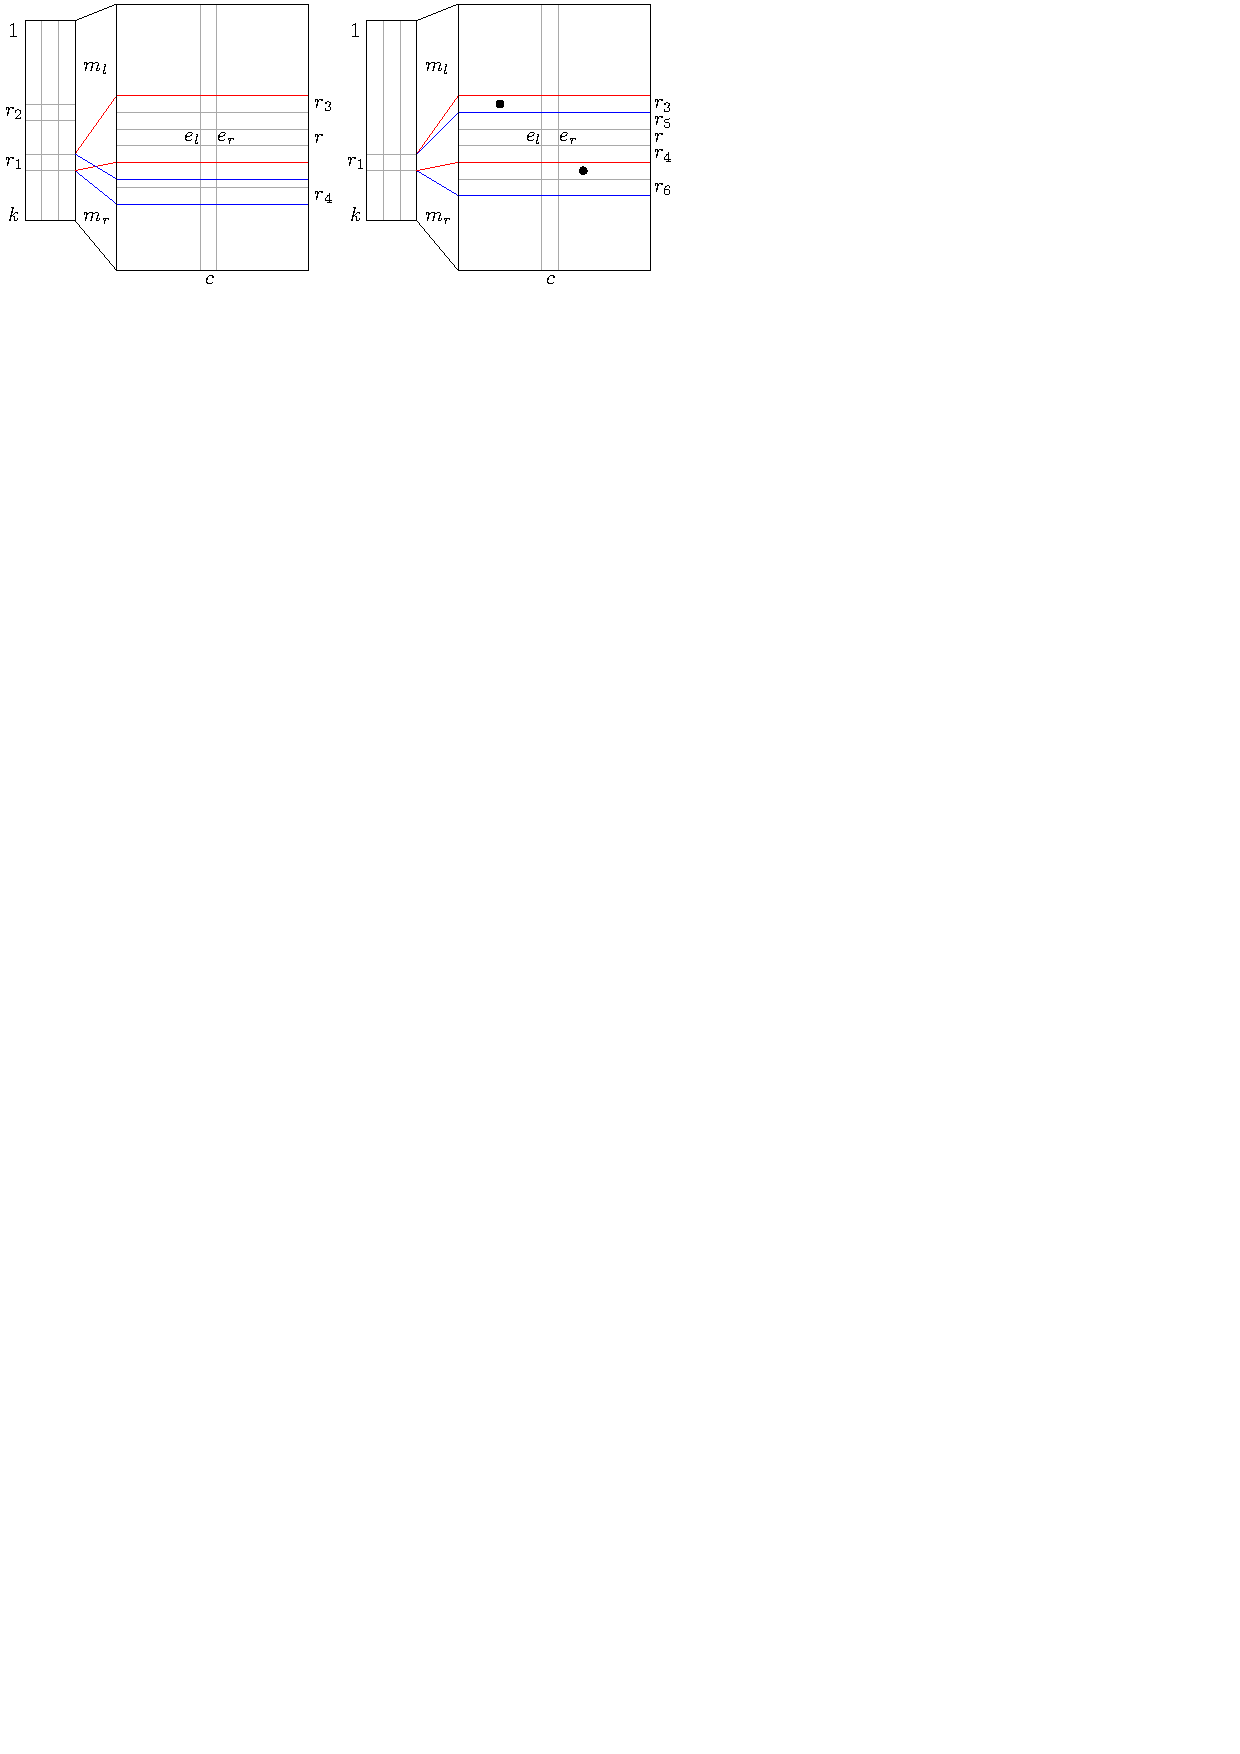
\includegraphics[width=\textwidth]{img/emptymidcol.pdf}
\caption{Red and blue lines representing mappings $m_l$ and $m_r$ of the forbidden pattern. The two horizontal lines show the boundaries of the mapping of row~$r$ and the vertical lines show the boundaries of the mapping of column~$c$.}
\label{fig:emptymid}
\end{figure}
\end{proof}

\begin{thm}
\label{thm:emptymiddle}
Let $P\in\bin^{k\times2}$ and for any integer $l\geq1$ let $P^l\in\bin^{k\times(l+2)}$ be a pattern created from $P$ by adding $l$ new empty columns in between the two columns of $P$. For all matrices $M\in\Mat$ it holds $M\in\Avm{P^l}\Leftrightarrow$ there exists a matrix $N\in\bin^{m\times(n-l)}$ such that $N\in\Avm{P}$ is critical and $M$ is a submatrix of an elementwise OR of $l+1$ shifted copies of $N$ ($N\hsum\{0\}^{m\times l},\{0\}^{m\times 1}\hsum N\hsum\{0\}^{m\times(l-1)},\dots,\{0\}^{m\times(l-1)}\hsum N\hsum\{0\}^{m\times1},\{0\}^{m\times l}\hsum N$).
\end{thm}
\begin{proof}
\begin{itemize}
	\item[$\Rightarrow$] Without loss of generality, let $M$ be critical. We know from Lemma~\ref{lemma:maxmult} that each row of $M$ contains either no one-entry or a single one-interval of length at least $l+1$. Let a matrix~$N$ be created from $M$ by deleting the last $l$ one-entries from each row and excluding the last $l$ columns. Clearly, $M$ is equal to an elementwise OR of $l+1$ copies of $N$. If $P\im N$ then each mapping of $P$ can be extended to a mapping of $P^l$ to $M$ by mapping each $P^l[r_1,1]$ to the same one-entry where $P[r_1,1]$ is mapped in $N\hsum\{0\}^{m\times l}$ and mapping each $P^l[r_2,l+2]$ to the same one-entry where $P[r_2,2]$ is mapped in $\{0\}^{m\times l}\hsum N$.
	\item[$\Leftarrow$] Let $M$ be equal to an elementwise OR of $l+1$ copies of $N$. For contradiction, assume $P^l\im M$ and consider any mapping of $P^l$ to $M$. Without loss of generality, one-entries of the first column of $P^l$ are mapped to those one-entries of $M$ created from $N\hsum\{0\}^{m\times l}$. If there is one-entry $P^l[r,1]$ mapped to a one-entry of $M$ not created from $N\hsum\{0\}^{m\times l}$, we just take the first one-entry in the row instead. Symmetrically, all one-entries of the last column of $P^l$ are mapped to one-entries created from $\{0\}^{m\times1}\hsum N$. The same one-entries of $N$ can be used to map $P$ to $N$, which is a contradiction.
\end{itemize}
\end{proof}

The symmetric characterization also holds when adding empty rows to a pattern that only has two rows. We can see in the following proposition that the straightforward generalization of the statement for bigger patterns does not hold.

\begin{prop}
There exists a matrix $P\in\Pat$ such that for each $P'\in\bin^{k\times(l+1)}$ created from $P$ by adding a single empty column in between two existing columns, there exists a matrix~$N$ avoiding $P$ such that the elementwise OR of $N\hsum\{0\}^{m\times 1}$ and $\{0\}^{m\times 1}\hsum N$ contains $P'$ as an interval minor.
\end{prop}
\begin{proof}
Later in this chapter, we characterize the class of matrices avoiding pattern~$P_8$. For the result, look at Proposition~\ref{prop:p72}. Let $N\in\Avm{P_8}$ be any matrix containing $P_5$ as an interval minor. Let a matrix $M$ be equal the elementwise OR of $N\hsum\{0\}^{m\times 1}$ and $\{0\}^{m\times 1}\hsum N$. Then $\smm{\bullet&\circ&\bullet&\bullet\\ &\circ&\bullet& },\smm{\bullet&\bullet&\circ&\bullet\\ &\bullet&\circ& }\im M$.
\end{proof}

Next, we describe the structure of matrices avoiding certain small patterns. We restrict ourselves to patterns with no empty lines. If $\PnimM$ then also $P^\top\nim M^\top$ and this holds for all rotations and mirrors of $P$ and $M$ and so we only mention these symmetries.

\section{Patterns having two one-entries and their generalization}
\label{sec:2ones}
These are, up to rotation and mirroring, the only patterns having two one-entries and no empty lines:
$$P_1=\smm{\bullet&\bullet}\ \ 
\ P_2=\smm{ &\bullet\\\bullet& }$$
They can be generalized to:
$$P'_1=\smm{\bullet&\bullet&\cdots&\bullet&\bullet}\ \ 
\ P'_2=\smm{ & & & &\bullet\\ & & &\bullet& \\ & &\Ddots& & \\ &\bullet& & & \\\bullet& & & & }$$

\begin{prop}
Let $P'_1=1^{1\times k}$. For all matrices $M$: $P'_1\nim M\Leftrightarrow M$ has at most $k-1$ non-empty columns.
\end{prop}
\begin{proof}
\begin{itemize}
	\item[$\Rightarrow$] When a matrix~$M$ contains one-entries in $k$ columns, then these give us a mapping of $P'_1$.
	\item[$\Leftarrow$] A matrix~$M$ having at most $k-1$ non-empty columns avoids $P'_1$.
\end{itemize}
\end{proof}

\begin{prop}
\label{prop:walking}
Let $P'_2\in\bin^{k\times k}$. For all matrices $M$: $P'_2\nim M\Leftrightarrow$ there are $k-1$ walks in $M$ such that each one-entry of $M$ belongs to at least one walk.
\end{prop}
\begin{proof}
\begin{itemize}
	\item[$\Rightarrow$] When one-entries of a matrix~$M$ cannot fit into $k-1$ walks, then there are $k$ one-entries such that no pair can fit to a single walk and those give us a mapping of $P'_2$.
	\item[$\Leftarrow$] A matrix~$M$ containing one-entries in at most $k-1$ walks avoids $P'_2$.
\end{itemize}
\end{proof}

\section{Patterns having three one-entries}
\label{sec:3ones}
These are up to rotation and mirroring the only patterns having three one-entries and no empty lines that we did not characterize so far:
$$P_3=\smm{\bullet&\bullet\\\bullet& }\ \ 
\ P_4=\smm{\bullet& &\bullet\\ &\bullet& }\ \ 
\ P_5=\smm{ &\bullet&\bullet\\\bullet& & }\ \ 
\ P_6=\smm{ &\bullet& \\\bullet& & \\ & &\bullet}$$

\begin{prop}
\label{prop:p31}
For all matrices $M\in\Mat$: $P_3\nim M\Leftrightarrow$ there exist a row~$r$ and a column~$c$ such that (see Figure~\ref{fig:p12}):
\begin{itemize}
\item $M[r,c]$ is top-left, top-right and bottom-left empty, and
\item $M[[r,m],[c,n]]$ is a walking matrix.
\end{itemize}
\end{prop}
\begin{figure}[!ht]
\centering
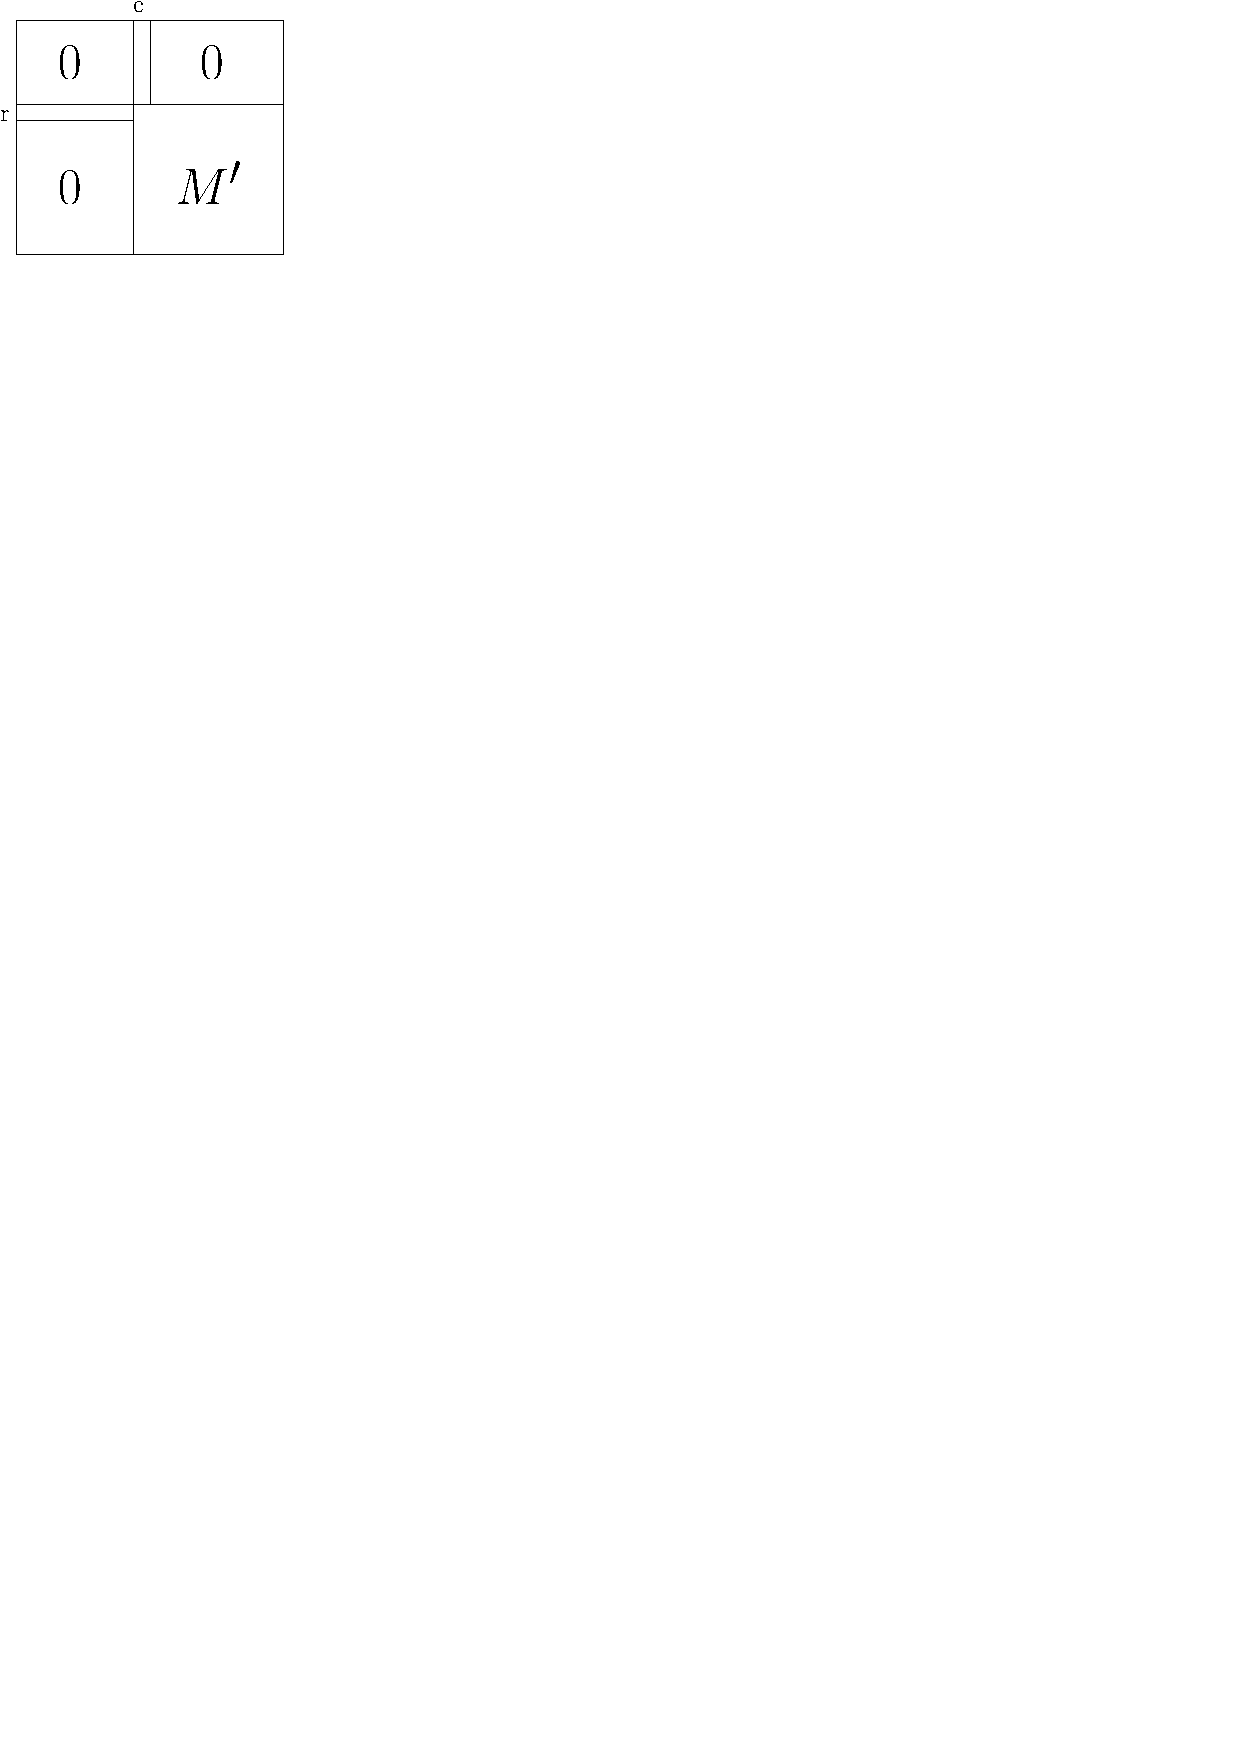
\includegraphics[width=50mm]{img/p12.pdf}
\caption{The characterization of matrices avoiding \usebox{\smlmat} as an interval minor. The matrix $M'$ is a walking matrix.}
\label{fig:p12}
\end{figure}
\begin{proof}
\begin{itemize}
	\item[$\Rightarrow$] If $M$ is a walking matrix then we set $r=c=1$. Otherwise, there are one-entries $M[r,c']$ and $M[r',c]$ such that $r'<r$ and $c'<c$. If $M[r,c]$ is not top-left, top-right or bottom-left empty then $\PimM$. If $M[[r,m],[c,n]]$ is not a walking matrix then it contains $\smm{ &\bullet\\\bullet& }$ and together with $M[r,c']$ it gives us the forbidden pattern.
	\item[$\Leftarrow$] For contradiction, assume that a matrix~$M$ described in Figure~\ref{fig:p12} contains $P_3$ as an interval minor. Without loss of generality, let $P_3[1,1]$ be mapped to a one-entry in the $r$-th row. Then both $P_3[1,2]$ and $P_3[2,1]$ need to be mapped to $M'$, which is a contradiction because it is not a walking matrix.
\end{itemize}
\end{proof}

\begin{prop}
For all matrices $M$: $P_4\nim M\Leftrightarrow M=M_1\hsum M_2$, where $\smm{\bullet& \\ &\bullet}\nim M_1$ and $\smm{ &\bullet\\\bullet& }\nim M_2$.
\end{prop}
\begin{proof}
\begin{itemize}
	\item[$\Rightarrow$] Let $e=M[r,c]$ be an arbitrary top-most one-entry in $M$. It holds $\smm{\bullet& \\ &\bullet}\nim M[[m],[c-1]]$, as otherwise, together with $e$ it forms $P_4$. If we also have $\smm{ &\bullet\\\bullet& }\nim M[[m],[c,n]]$ then we are done. For contradiction, let $e_1,\ e_2$ be any two one-entries forming $\smm{ &\bullet\\\bullet& }$ in $M[[m],[c,n]]$. Symmetrically, let $e'_1,\ e'_2$ be any two one-entries forming $\smm{\bullet& \\ &\bullet}$ in $M[[m],[c]]$. Without loss of generality, let $e_2$ be lower than $e'_2$ and then, together with $e'_1$ and $e_1$ it forms $P_4$ as an interval minor of $M$, giving us a contradiction. 
	\item[$\Leftarrow$] For contradiction, let $P_4\im M$ and consider an arbitrary mapping. Consider the one-entry of $M$, where $P_4[2,2]$ is mapped. If it is in $M_1$ then $\smm{\bullet& \\ &\bullet}\im M_1$ and we get a contradiction. Otherwise, we have $\smm{ &\bullet\\\bullet& }\im M_2$, which is again a contradiction.
\end{itemize}
\end{proof}

\begin{prop}
For all matrices $M\in\Mat$: $P_5\nim M\Leftrightarrow$ for every one-entry $M[r,c]$ on the bottom-left extreme walk~$w$, there is at most one non-empty column in $M[[r-1],[c+1,n]]$.
\end{prop}
\begin{proof}
\begin{itemize}
	\item[$\Rightarrow$] For contradiction, assume there is a one-entry~$M[r,c]$ on $w$ such that there are two non-empty columns in $M[[r-1],[c+1,n]]$. Then a one-entry from each of those columns and $M[r,c]$ together give us $P_5\im M$ and a contradiction. 
	\item[$\Leftarrow$] For contradiction, let $P_5\im M$. Without loss of generality, $P_5[2,1]$ is mapped to a one-entry~$M[r,c]$ from $w$. Then $\smm{\bullet&\bullet}\im M[[r-1],[c+1,n]]$, which is a contradiction with it having one-entries in at most one column.
\end{itemize}
\end{proof}

\begin{prop}
For all matrices $M$: $P_6\nim M\Leftrightarrow$ for every one-entry $M[r,c]$ on the bottom-right extreme reverse walk~$w$, $M[[r-1],[c-1]]$ is a walking matrix.
\end{prop}
\begin{proof}
\begin{itemize}
	\item[$\Rightarrow$] For contradiction, assume there are $r,c$ such that $M[r,c]$ is a one-entry on $w$ and $M[[r-1],[c-1]]$ is not a walking matrix. It means that $\smm{ &\bullet\\\bullet& }\im M[[r-1],[c-1]]$ and together with $M[r,c]$ it gives us the forbidden pattern and a contradiction.
	\item[$\Leftarrow$] For contradiction, let $P_6\im M$ and consider an arbitrary mapping of $P_6$. Without loss of generality, let $P_6[3,3]$ be mapped to $M[r,c]$ such that there is no other one-entry in $M[[r,m],[c,n]]$. Then, $M[r,c]$ lies on $w$ and $M[[r],[c]]$ is a walking matrix and so $M[r,c]$ cannot be used to map $P_6[3,3]$, which is a contradiction.
\end{itemize}
\end{proof}

\section{Patterns having four one-entries}
\label{sec:4ones}
These are some of the patterns having four one-entries and no empty lines that we did not characterize so far:
$$P_7=\smm{\bullet&\bullet\\\bullet&\bullet}\ \ 
\ P_8=\smm{\bullet&\bullet&\bullet\\ &\bullet& }\ \ 
\ P_9=\smm{ &\bullet& & \\\bullet& & & \\ & & &\bullet\\ & &\bullet& }$$

\begin{lemma}
\label{lemma:p33}
For any matrix $M$: $P_7\nim M\Rightarrow$ there exist integers $r,c$ such that $M[r,c]$ is either
\begin{enumerate}
\item a one-entry and $(r,c)\in\{(1,1),(1,n),(m,1),(m,n)\}$ or
\item top-right and bottom-left empty and $(r,c)\not\in\{(1,1),(m,n)\}$ or
\item top-left and bottom-right empty and $(r,c)\not\in\{(1,n),(m,1)\}$.
\end{enumerate}
\end{lemma}
\begin{proof}
If there is a one-entry in any corner then the first condition is satisfied. Otherwise, consider $M[2,1]$. It is trivially bottom-left empty and if there is no one-entry in the first row of $M$ then the second condition is satisfied. Therefore, let $M[1,c_t]$ be a one-entry in the first row. Symmetrically, let $M[m,c_b]$ be a one-entry in the last row, let $M[r_l,1]$ be a one-entry in the first column and let $M[r_r,n]$ be a one-entry in the last column.

It cannot happen that $c_t<c_b$ and $r_r>r_l$ (or symmetrically $c_t>c_b$ and $r_r<r_l$), because then $P_7\im M$. Without loss of generality, let $c_t\geq c_b$ and $r_r\geq r_l$. The matrix $M[[r_r-1],[c_t+1,n]]$ is empty; otherwise, any one-entry there, together with $M[1,c_t],M[m,c_b]$ and $M[r_r,1]$ forms the forbidden pattern. Similarly, the matrix $M[[r_r+1,m],[c_t-1]]$ is also empty. Thus $M[r_t,c_t]$ is top-right and bottom-left empty and it is not a corner, because those are empty.
\end{proof}

\begin{prop}
\label{prop:p33}
For all matrices $M\in\Mat$: $P_7\nim M\Leftrightarrow$ there are integers $r,c$ such that either (see Figure~\ref{fig:p33})
\begin{enumerate}
	\item $M[r,c]$ is top-right empty and bottom-left empty, $\smm{\bullet&\bullet\\\bullet& }\nim M[[r],[c]]$ and $\smm{ &\bullet\\\bullet&\bullet}\nim M[[r,m],[c,n]]$, or
	\item $M[r,c]$ is top-left empty and bottom-right empty, $\smm{\bullet&\bullet\\ &\bullet}\nim M[[r],[c,n]]$ and $\smm{\bullet& \\\bullet&\bullet}\nim M[[r,m],[c]]$.
\end{enumerate}
\end{prop}
\begin{figure}[!ht]
\centering
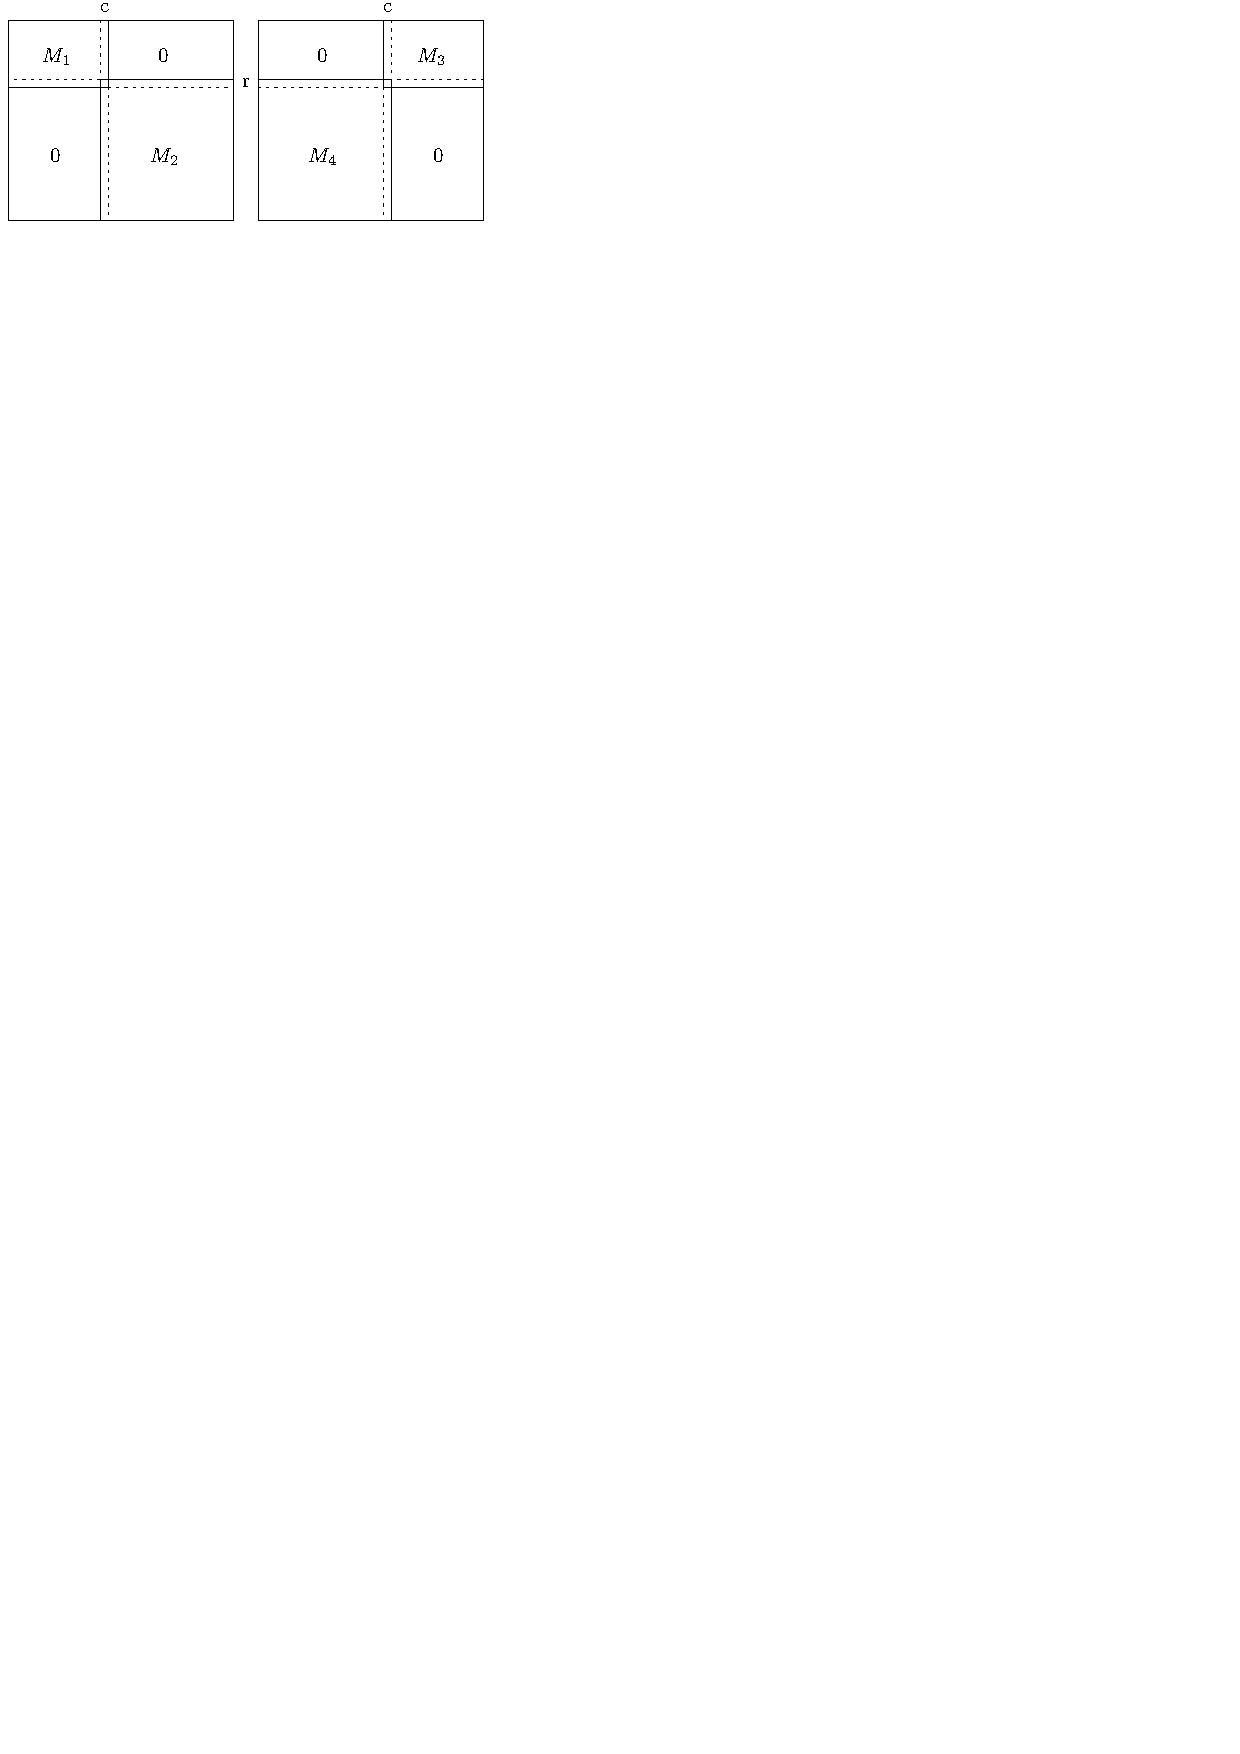
\includegraphics[width=100mm]{img/p33.pdf}
\caption{The characterization of matrices avoiding \usebox{\smlmatb} as an interval minor.}
\label{fig:p33}
\end{figure}
\begin{proof}
We let $M_1=M[[r],[c]],\ M_2=M[[r,m],[c,n]],\ M_3=M[[r],[c,n]]$ and $M_4=M[[r,m],[c]]$.
\begin{itemize}
	\item[$\Rightarrow$] We proceed by induction on the size of $M$.

If $M\in\bin^{2\times2}$ then it either avoids $\smm{ &\bullet\\\bullet&\bullet}$ or $\smm{\bullet&\bullet\\\bullet& }$ and we are done.

For a bigger matrix $M$, from Lemma~\ref{lemma:p33}, there is an element $M[r,c]$ satisfying some conditions. If there is a one-entry in any corner, we are done because the matrix cannot contain one of the rotations of $\smm{\bullet&\bullet\\\bullet& }$. Otherwise, assume $M[r,c]$ is both top-right and bottom-left empty and $(r,c)\not\in\{(1,1),(1,1)\}$. Let $M_1=M[[r],[c]]$ and $M_2=M[[r,m],[c,n]]$. If $M_1$ is non-empty, then $\smm{ &\bullet\\\bullet&\bullet}\nim M_2$. Symmetrically, $\smm{\bullet&\bullet\\\bullet& }\nim M_1$ if $M_2$ is non-empty. If one of them is empty, the other is a smaller matrix avoiding $P$ as an interval minor and the statement follows from the induction.
	\item[$\Leftarrow$] Without loss of generality, assume a matrix $M$ looks like the left matrix in Figure~\ref{fig:p33}. For contradiction, let $\PimM$. We can partition $M$ into four quadrants such that there is at least one one-entry in each of them. It does not matter where we partition it, every time we either get $\smm{\bullet&\bullet\\\bullet& }\im M_1$ or $\smm{ &\bullet\\\bullet&\bullet}\im M_2$, which is a contradiction.
\end{itemize}
\end{proof}

\begin{lemma}
\label{lemma:p72}
For all matrices $M$: $P_8\nim M\Rightarrow M=M_1\hsum M_2$ where
\begin{enumerate}
\item $\smm{\bullet&\bullet\\ &\bullet}\nim M_1$ and $\smm{ &\bullet\\\bullet& }\nim M_2$ or
\item $\smm{\bullet& \\ &\bullet}\nim M_1$ and $\smm{\bullet&\bullet\\\bullet& }\nim M_2$.
\end{enumerate}
\end{lemma}
\begin{proof}
Let $e=M[r,c]$ be an arbitrary top-most one-entry of $M$. It holds $\smm{\bullet&\bullet\\ &\bullet}\nim M[[m],[c-1]]$; otherwise, together with $e$ it would form the whole $P_8$. Symmetrically, $\smm{\bullet&\bullet\\\bullet& }\nim M[[m],[c+1,n]]$. For contradiction with statement, let $e_1,\ e_2$ (none of them equal to $e$) be any two one-entries forming $\smm{\bullet& \\ &\bullet}$ in $M[[m],[c]]$ and let $e'_1,\ e'_2$ be any two one-entries forming $\smm{ &\bullet\\\bullet& }$ in $M[[m],[c,n]]$. Without loss of generality, $e'_2$ is lower than $e_2$ and together with $e_1,\ e$ and $e'_1$ it gives us a mapping of $P_8$ to $M$, which is a contradiction.
\end{proof}

\begin{prop}
\label{prop:p72}
For all matrices $M\in\Mat$: $P_8\nim M\Leftrightarrow$ there are integers $r,c_1$ and $c_2$ such that all one-entries of $M$ above the row~$r$ are in columns $c_1$ and $c_2$, $M[[r+1,m],[c_1+1,c_2-1]]$ is empty, $\smm{\bullet& \\ &\bullet}\nim M[[r,m],[c_1]]$ and $\smm{ &\bullet\\\bullet& }\nim M[[r,m],[c_2,n]]$. See Figure~\ref{fig:p72}.
\end{prop}
\begin{figure}[!ht]
\centering
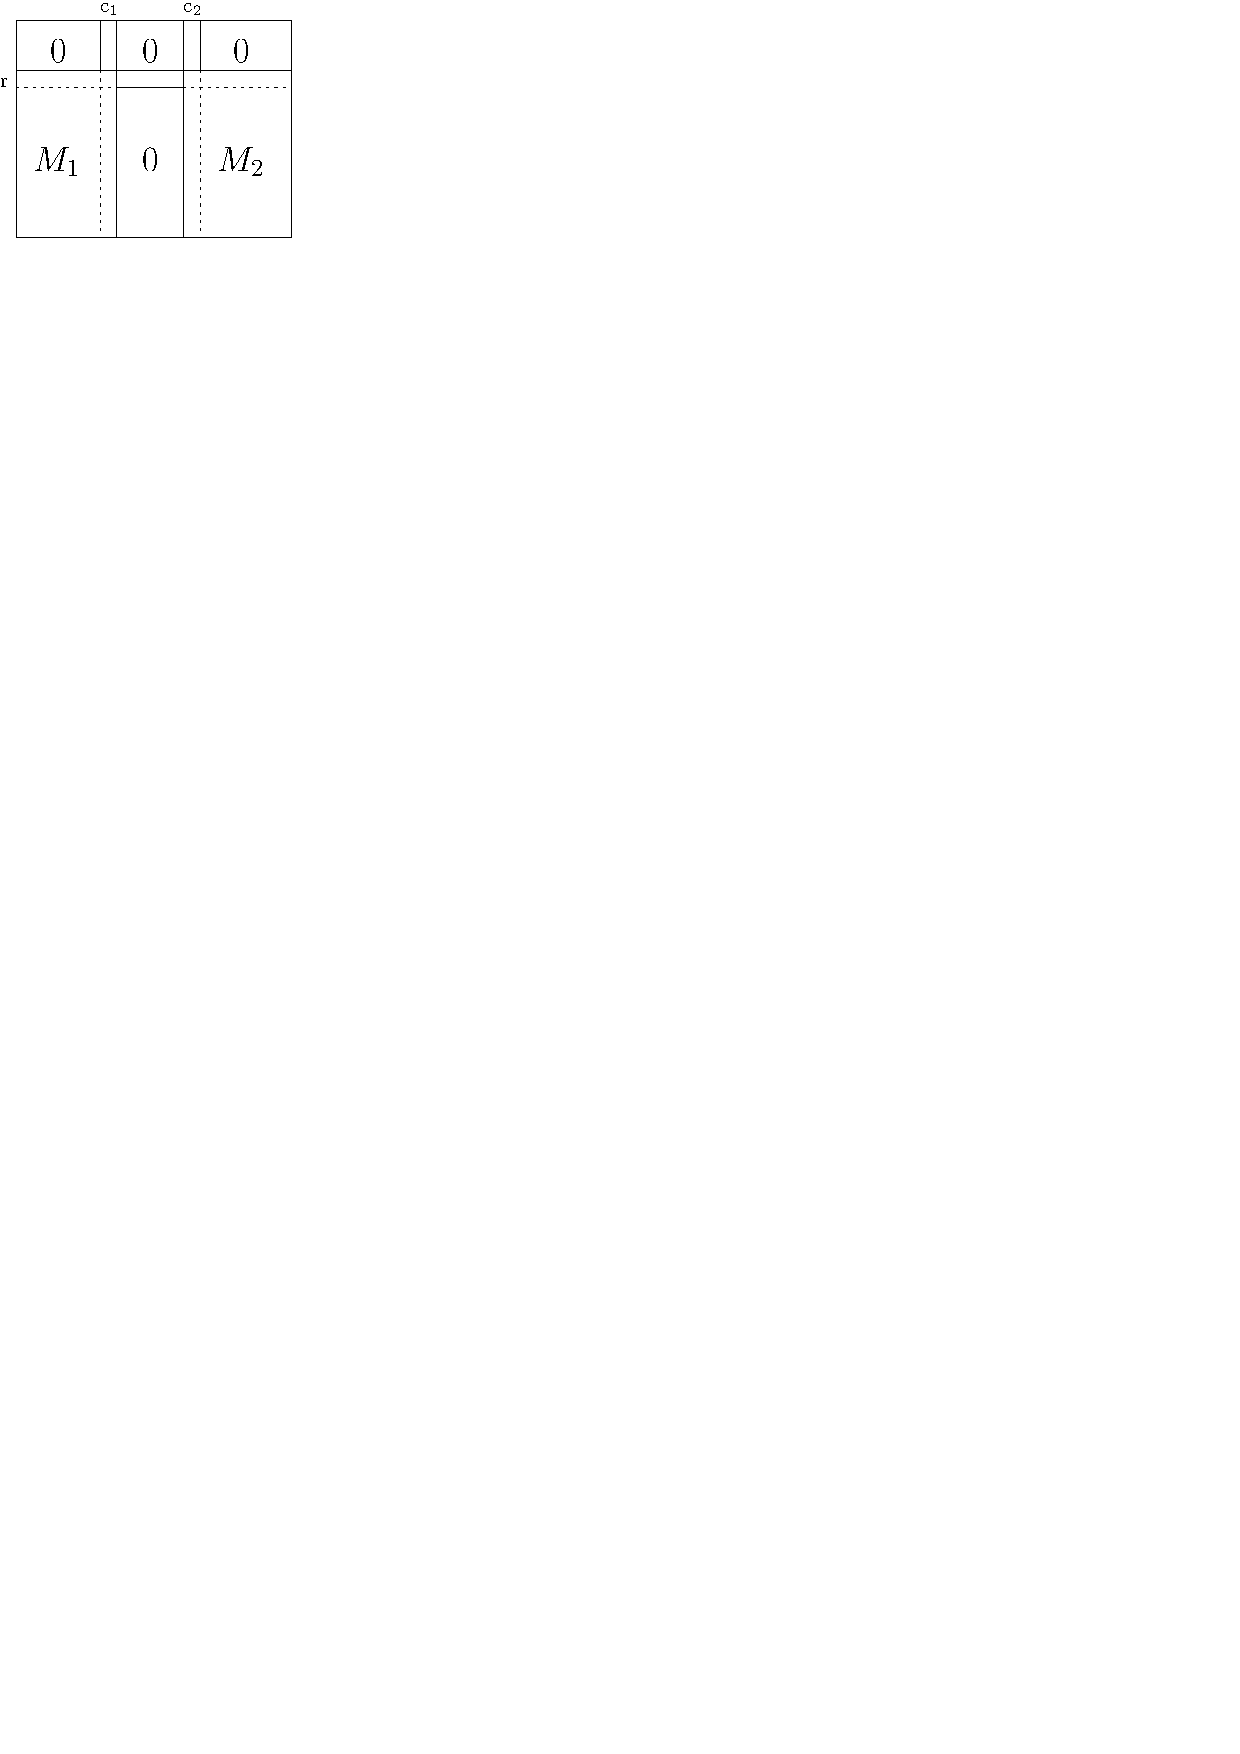
\includegraphics[width=60mm]{img/p72.pdf}
\caption{The characterization of matrices avoiding \usebox{\smlmatc} as an interval minor.}
\label{fig:p72}
\end{figure}
\begin{proof}
\begin{itemize}
	\item[$\Rightarrow$] From Lemma~\ref{lemma:p72}, we know $M=M_1'\hsum M_2'$, where $\smm{\bullet&\bullet\\ &\bullet}\nim M_1'$ and $\smm{ &\bullet\\\bullet& }\nim M_2'$ (or symmetrically the second case). From Proposition~\ref{prop:p31}, we have that $M_1'$ looks like $M[[m],[c_2-1]$ in Figure~\ref{fig:p72} and $M[[m],[c_2,n]]$ forms a walking matrix. Without loss of generality, $M[[r-1],\{c_1\}]$ and $M[\{r\},[c_1+1,c_2-1]]$ are non-empty; otherwise, we extend $M_1$ to cover the whole $M[[m],[c_2-1]$. If there are two different columns in $M_2'$ having a one-entry above the $r$-th row, together with one-entries in $M[[r-1],\{c_1\}]$ and $M[\{r\},[c_1+1,c_2-1]]$ they form a mapping of $P_8$.
	\item[$\Leftarrow$] A one-entry~$P_8[2,2]$ can not be mapped anywhere but to the $r$-th row, but in that case, there are at most two columns having one-entries above it.
\end{itemize}
\end{proof}

\section{Multiple patterns}
Instead of considering matrices avoiding a single pattern, we can work with matrices avoiding a set of forbidden patterns.

We only describe the structure of matrices avoiding one particular set of patterns, because we use the simple result later.

\begin{prop}
\label{prop:twopatterns}
Let $P_{10}=\smm{\circ&\circ&\bullet\\\bullet&\circ&\circ}$ and $P_{11}=\smm{\circ&\bullet\\\circ&\circ\\\bullet&\circ}$, then for all matrices $M$: $\{P_{10},P_{11}\}\nim M\Leftrightarrow$ for the bottom-left extreme walk~$w$ in $M$, each one-entry $M[r,c]$ is either on $w$ or both $M[r+1,c]$ and $M[r,c-1]$ are on $w$.
\end{prop}
\begin{proof}
\begin{itemize}
	\item[$\Rightarrow$] For contradiction, assume there is a one-entry anywhere but on $w$ or directly diagonally next to any bottom-left corner of $w$. Then this one-entry together with at least one bottom-left corner of $w$ give us a mapping of $P_{10}$ or $P_{11}$ and a contradiction.
	\item[$\Leftarrow$] For any one-entry~$e$, from the description of $M$, there is no one-entry that creates $P_{10}$ or $P_{11}$ with $e$.
\end{itemize}
\end{proof}